\chapter{Društvene mreže i zajednice}

Društvene mreže može se pronaći gdje god postoji sustav koji sadrži entitete koji su međusobno povezani. Primjera je mnogo, a neki od njih su: društvene web platforme, email mreža, web stranice koje sadrže poveznice prema dugima, uređaji koji su povezani preko internetske mreže i slično. 
Kako bi se skupina entiteta mogla nazvati društvenom zajednicom među njima mora postojati nekakav tip odnosa. Može biti jednosmjerni ili dvosmjerni te mogu postojati težine kojima se odnosu daje veća ili manja značajnost. Društvene mreže imaju složenu organizacijsku strukturu te se može pretpostaviti svojstvo lokalnosti koje kaže da ako jedan entitet ima veze prema neka druga dva entiteta onda je vjerojatnost da ta druga dva entiteta imaju vezu veća od prosječne. 

Društvene mreže imaju karakteristično svojstvo grupiranja u strukturu zajednice. Ako se čvorovi mreže mogu podijeliti u nepreklapajuće ili preklapajuće zajednice tako da broj veza između članova zajednice značajno premašuje broj veza između bilo koje dvije zajednice znači da mreža ima strukturu društvenih zajednica. Mreže koje imaju takvu strukturu često se mogu prikazati i kao hijerarijske strukture. U ovom radu obradit će se mreže koje sadrže nepreklapajuće strukture sa vezama koje nemaju određene težine.

Proces pronalaska društvenih zajednica jedan je od glavnih zadataka u analizama društvenih mreža. Detekcija zajednica može biti vrlo korisna u raznim primjenama kao što je primjerice pronalaženje grupa kojima bi se mogle slati reklame za određene proizvode koji bi ih mogli zanimati umjesto da se svakom pojedincu šalju posebno. Još jedan primjer bio bi preporuka određenih sadržaja koji bi se mogli prikazivati grupama koje pokazuju zanimanja prema sličnim interesima. Primjera ima još mnogo, ali iz ova dva je već vidljivo da se korisne informacije mogu zaključivati iz društvenih mreža. Kako bi društvene mreže pohranili i analizirali u računalu potrebna je prikladna struktura podataka koja će u ovom slučaju biti graf.

\section{Reprezentacija društvenih mreža}
Prema definiciji jednostavan graf \textit{G} sastoji se od nepraznog konačnog skupa \textit{V(G)}, čije se elemente naziva vrhovi ili čvorovi grafa i konačnog skupa \textit{E(G)} različitih dvočlanih podskupova skupa \textit{V(G)} koji se naziva bridovima \cite{nakic_pavcevic_2019}. Graf može imati najviše $ {n(n-1) \over 2} $. U radu će se razmatrati jednostavni grafovi koji nemaju petlje i više bridova između istih čvorova. Bridovi će biti bestežinski i neusmjereni. 

Bitna definicija tiče se stupnja vrhova grafa. Stupanj vrha \textit{v} grafa \textit{G} je broj bridova koji su incidentni s \textit{v}. Stupanj vrha označava se sa \textit{deg(v)}. Vrh stupnja 0 zove se izolirani vrh, a vrh stupnja 1 krajnji vrh. \cite{nakic_pavcevic_2019}

Šetnja je graf sa skupom vrhova \textit{V(G) = $ \{x_{1},x_{2},...,x_{l}\} $ } i bridova \textit{E(G) = $ \{x_{0}x_{1},x_{1}x_{2},...,x_{l-1}x_{l}\} $ }. vrhovi $ x_{0} $ i $ x_{l} $ definiraju se kao krajevi dok je \textit{l} duljina šetnje. Ako su svi bridovi šetnje različiti tada se ona naziva staza. Ako su uz to i svi vrhovi različiti onda se takva šetnju naziva putem. Ako put počinje i završava u istom vrhu tada graf sadrži ciklus. Uz pretpostavljena ograničenja najmanji ciklus koji graf u ovom radu može imati je trokut što je često obilježje društvenih mreža.

Definicija puta omogućava definiranje važnog koncepta koji će se pojavljivati u radu pojedinih algoritama. Ako u grafu za svaki par vrhova postoji barem jedan put koji ide od jednog do drugog onda je graf povezan. Ako između vrhova postoji više putova onda je najkraći onaj koji ima najmanju duljinu. Promjer ili dijametar povezanog grafa je najveća udaljenost između bilo koja dva vrha u grafu. Ako ipak postoji barem jedan par vrhova između kojih ne postoji put onda je graf podijeljen u barem dva podgrafa. Svaki maksimalno povezani podgraf zove se komponenta povezanosti. Primjer se može vidjeti na slici \ref{fig:graph}.

\begin{figure}
	\makebox[\textwidth][c]{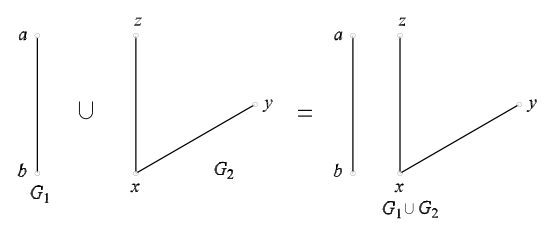
\includegraphics[width=0.7\textwidth]{images/nepovezani-graf.png}}
	%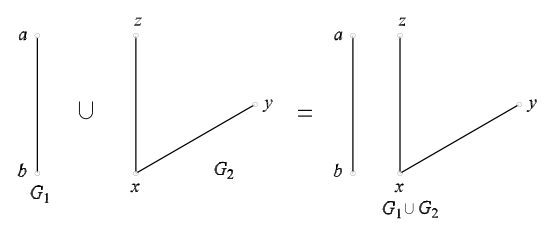
\includegraphics[width=0.7\textwidth]{images/nepovezani-graf.png}
	\caption{Primjer nepovezanog grafa}
	\label{fig:graph}
\end{figure}

Grafovi se mogu pohranjivati u obliku matrice susjedstva gdje su dva vrha, \textit{i} i \textit{j} susjedna ako im je element matrice \textit{A{ij}} jednak 1, a inače 0. Zbog pretpostavke da ne postoje petlje na dijagonali matrice susjedstva svi su elementi nule. Za reprezentaciju neusmjerenog grafa matrica susjedstva je simetrična što znači da je dovoljno pohraniti samo jedan trokut matrice, iznad ili ispod dijagonale. Suma elemenata \textit{i}-tog retka ili stupca jednaka je stupnju vrha \textit{i}

Jednostavniji oblik pohrane koji zauzima manje prostora u datoteci je takav da se pohranjuje popis bridova grafa te se i on može koristiti.


\section{Obilježja društvenih zajednica} 

Društvene zajednice moguće je definirati na nekoliko načina sa različitih stajališta, ali ne postoji niti jedna univerzalno prihvaćena definicija. Definiranje vrlo često ovisi o problemu koji se promatra zajedno sa specifičnim detaljima i primjenama gdje se pojam zajednice koristi. Prema radu \cite{fortunato2010community} zajednice je moguće promatrati iz lokalne i globalne perspektive.

Iz lokalne perspektive zajednica se može promatrati kao grupa entiteta koji su međusobno sličniji u odnosu na ostale entitete skupa podataka. Zajednica se formira tako što slični elementi imaju mnogo više interakcija sa članovima unutar zajednice u odnosu na one izvan. Zajednica se može smatrati kao autonomna skupina te ima smisla u određenim situacijama evaluirati svaku zasebno od ostatka društvene mreže. Stroga definicija društvene mreže kaže kako je društvena zajednica podgraf u kojem su svi članovi međusobno u interakciji \cite{luce1949method}. Takva definicija odgovara terminu klike u teoriji grafova koji označava skup vrhova koji su svi međusobno susjedni. Najjednostavniji primjer klike je trokut i oni se pojavljuju u svim društvenim mrežama. Veće klike od trokuta se pojavljuju rjeđe te ovakva definicija tako postaje manje praktična u stvarnim primjerima. Još jedan problem klike je to su tada svi vrhovi simetrični bez mogućnosti razlikovanja njihovih svojstava. U praktičnim primjerima očekuje se da među vrhovima postoji određena hijerarhijska struktura sa više i manje važnim čvorovima. Moguće je relaksirati pojam klike. Mogućnost je iskoristiti doseg i duljinu puta između čvorova. n-klika je takav podgraf da niti jedan par vrhova nije međusobno udaljen za više od \textit{n} koraka i skup je maksimalan u smislu da niti jedan drugi čvor nije udaljen za više od \textit{n} od svakog čvora iz podgrafa. Može se primijetiti da članovi podgrafa mogu biti povezani preko posrednika koji nije član grupe te onda n-klika ipak nije dovoljno dobra definicija. Definicija n-klana to popravlja. n-klan je n-klika u kojoj je dijametar podgrafa manji ili jednak \textit{n}. Takva definicija ima problem što u njoj i dalje postoji zahtjev n-klike te se tako dolazi do definicije n-kluba. n-klub je podgraf gdje je dijametar manji ili jednak \textit{n}. Tada je i svaki n-klan i n-klub i n-klika.

Iz globalne perspektive zajednica se može definirati promatrajući graf u cjelini. Takve definicije koriste se u slučajevima kada su zajednice dijelovi sustava bez kojih bi njegovo funkcioniranje bilo značajno. Definicije se najčešće izvode indirektno, iz algoritma prema kojem je neko svojstvo iskorišteno kako bi se zajednice otkrile. 

\section{Small-world svojstvo}

Društvene mreže posjeduju small-world svojstvo što znači da bilo koja dva entiteta imaju kratku međusobnu udaljenost. Specifično je što se ona za dva slučajno izabrana čvora te za fiksiran prosječan stupanj vrha povećava proporcionalno logaritmu broj čvorova u grafu dok koeficijent grupiranja nije malen. 

Koeficijent grupiranja je mjera stupnja u kojem čvorovi u grafu teže grupiranju. Postoje dvije verzije mjere, lokalna i globalna. U lokalnoj verziji mjera se računa za pojedini čvor te govori u kolikoj je on mjeri grupiran sa svojim susjedima. Mjera se za čvor \textit{i} računa kao suma broja veza koje postoje između susjeda promatranog čvora podijeljeno sa brojem svih mogućih veza, $ C_{i} = \dfrac{2 \mid e_{jk}:v_{j},v_{k} \in N_{i}, e_{jk} \in E \mid}{k_{i}(k_{i}-1)} $. Ako iz formule maknemo koeficijent 2 tada se ona može koristiti za usmjerene grafove.
Globalni koeficijent grupiranja daje informaciju o grupiranju u cijeloj društvenoj mreži. Temelji se na trojkama čvorova. Trojku čine promatrani čvor i druga dva čvora. Ako su povezani sa dva brida zovu se otvorena trojka, a ako su povezani sa tri zovu se zatvorena trojka što znači da jedan trokut čine tri trojke. Koeficijent se tada računa kao broj zatvorenih trojki podijeljen sa ukupnim brojem trojki, $ C = \dfrac{broj \; zatvorenih \; trojki}{ukupan \; broj \; trojki} $. Formula je primjenjiva i na usmjerene i neusmjerene grafove.